\section{Abgrenzung des Projektes}
In diesem Kapitel soll eine Konzeptabgrenzung des Projektes gegenüber einem konventionellen Güterwagen, anderen bereits vorhandenen Lösungen und dem späteren vollständig ausgebildeten \gls{Gueterwagen 40} stattfinden. Dafür ist dieses Kapitel in die folgenden drei Unterkapitel geteilt.

\subsection{Railmap}
Bereits in Vorträgen, zum Beispiel auf der 1. BME-VDV-Gleisanschlusskonferenz \cite{GAK}, kam es zur Vorstellung der sogenannten Railmap, siehe Abbildung \ref{fig:Railmap}, diese zeigt einen Vorschlag für zukünftige Entwicklungen im Schienengüterverkehr. Auf ihr ist der Weg abgebildet, den unter anderem auch der \gls{Gueterwagen 40}  gehen soll, aber auch weitere Punkte, die danach für die Automatisierung des Schienengüterverkehrs folgen sollen.\par
\begin{figure}[hbp]
    \centering
    \definecolor{red1}{RGB}{228,26,28}
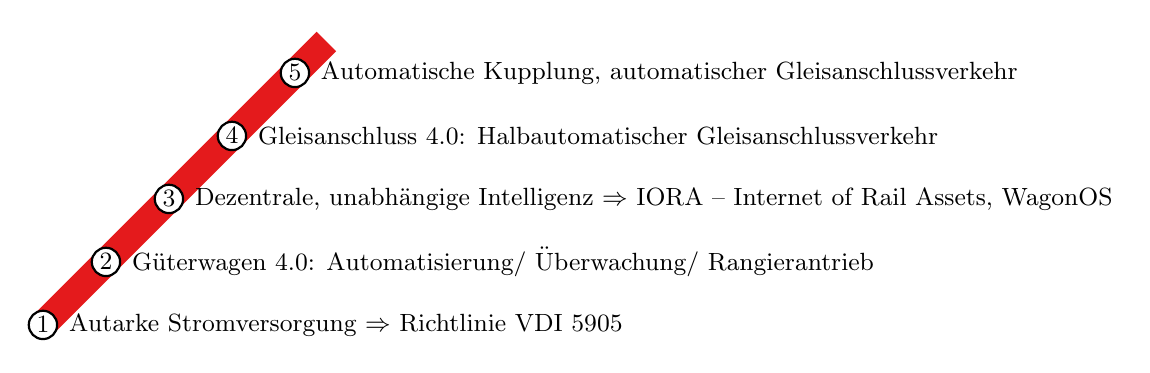
\begin{tikzpicture}[font = \sffamily, scale = 0.8]
\tikzstyle{every node}=[font=\small]
\path[line width = .35cm, draw = red1] (0,0) -- (4.5,4.5);
\path[draw, thick, fill = white] (0,0) node[circle, draw, fill = white, inner sep = 1] {1}  node[xshift = .2cm, anchor = west] {Autarke Stromversorgung $\Rightarrow$ Richtlinie VDI 5905};
\path[draw, thick, fill = white] (1,1) node[circle, draw, fill = white, inner sep = 1] {2} node[xshift = .2cm, anchor = west] {Güterwagen 4.0: Automatisierung/ Überwachung/ Rangierantrieb};
\path[draw, thick, fill = white] (2,2) node[circle, draw, fill = white, inner sep = 1] {3}  node[xshift = .2cm, anchor = west] {Dezentrale, unabhängige Intelligenz $\Rightarrow$ IORA -- Internet of Rail Assets, WagonOS};
\path[draw, thick, fill = white] (3,3) node[circle, draw, fill = white, inner sep = 1] {4}  node[xshift = .2cm, anchor = west] {Gleisanschluss 4.0: Halbautomatischer Gleisanschlussverkehr};
\path[draw, thick, fill = white] (4,4) node[circle, draw, fill = white, inner sep = 1] {5}  node[xshift = .2cm, anchor = west] {Automatische Kupplung, automatischer Gleisanschlussverkehr};
\end{tikzpicture}
    \caption{Railmap - angelehnt an \cite{GAK}}
    \label{fig:Railmap}
\end{figure}
Die Railmap beginnt mit dem Hauptpunkt, der auch ein Schwerpunkt dieses Projektes sein soll, der autarken Stromversorgung des Wagens. Dieser wird unter anderem mit der Erstellung der Richtlinie VDI 5905\footnote{www.vdi.de/5905 VDI 5905 Blatt 1 Schnittstellen aktiver, kooperierender Güterwagen - Stromversorgung} gefestigt.\par
Der zweite Punkt der Railmap besteht aus zwei Unterpunkten. Beide Punkte zusammen bilden den voll ausgestatteten \gls{Gueterwagen 40} wie er in Kapitel \ref{sec:Ausbaustufen} gezeigt wird. %\\
Der Unterpunkt 2a beschreibt den \gls{Gueterwagen 40} nach diesem Projekt. Darin enthalten ist die Ausstattung mit den Ausbaustufen 1 - Stromversorgung, 2 - Automatisierung der Bremse und 3 - die ep-''light''-Bremse. %\\
Der Unterpunkt 2b beschreibt die Ausbaustufen 4 und 5 des \gls{Gueterwagen 40} und damit die Einführung einer technischen Sicherung der Zugintegrität bei Güterwagen sowie des Rangierantriebs. Siehe dazu auch die einzelnen Punkte des Kapitels \ref{sec:Ausbaustufen}.\par
Als Drittes ist eine dezentrale, unabhängige Intelligenz von Güterwagen geplant. Diese soll dem Internet of Things entsprechen; dem Internet of Rail Assets. In diesem Punkt soll es für den Güterwagen möglich sein mit anderen 'Dingen' der Eisenbahn zu kommunizieren.\par
Im vierten Punkt geht es um halbautomatisierten Gleisanschlussverkehr und den sogenannten Gleisanschluss 4.0. auch hierzu gibt es bereits vorgestellte Ideen; wie zum Beispiel auf der 1. BME-VDV-Gleisanschlusskonferenz \cite{GAK}. \par
Im fünften und letzten Punkt dieser Railmap soll die automatische Kupplung flächendeckend eingeführt und ein automatischer Gleisanschlussverkehr möglich sein.\par
In diesem Projekt sollen \gls{konventionelle Gueterwagen} mit konventionellen Fahrwerken und Luftbremse zu \gls{Demonstrator}en umgebaut werden. Ein zusätzlicher Aufbau von Leistungs- und sicherheitsgerichteten Komponenten ist geplant, ebenso eine erste Realisierung der Bremse 4.0\cite{Stephenson, ETR_2}.\par

\subsection{Beschreibung der Ausbaustufen}\label{sec:Ausbaustufen}
Anhand des Ist- und Soll-Zustandes (siehe voriges und folgendes Kapitel) sind fünf Ausbaustufen für den \gls{Gueterwagen 40} geplant, die diese Zeiteinsparung bringen sollen. In den folgenden Abschnitten werden die geplanten Ausbaustufen kurz beschrieben.\par

\subsubsection{Ausbaustufe 1: Stromversorgung, Telematik und Datenvernetzung}
\begin{figure}[hbp] 
    \begin{comment}
\definecolor{class1}{RGB}{228,26,28}
\definecolor{class2}{RGB}{55,126,184}
\definecolor{class3}{RGB}{77,175,74}
\definecolor{class4}{RGB}{152,78,163}
\definecolor{class5}{RGB}{255,127,0}

\tikzset{wagon/.style={draw = gray, ultra thick, opacity = 0.7}}
\tikzset{class1/.style={draw = class1, ultra thick, opacity = 1}}
\tikzset{class2/.style={draw = class2, ultra thick, opacity = 1}}
\tikzset{class3/.style={draw = class3, ultra thick, opacity = 1}}
\tikzset{class4/.style={draw = class4, ultra thick, opacity = 1}}
\tikzset{class5/.style={draw = class5, ultra thick, opacity = 1}}
\tikzset{annotation/.style={draw = black, thick, opacity = 0.7}}
\end{comment}

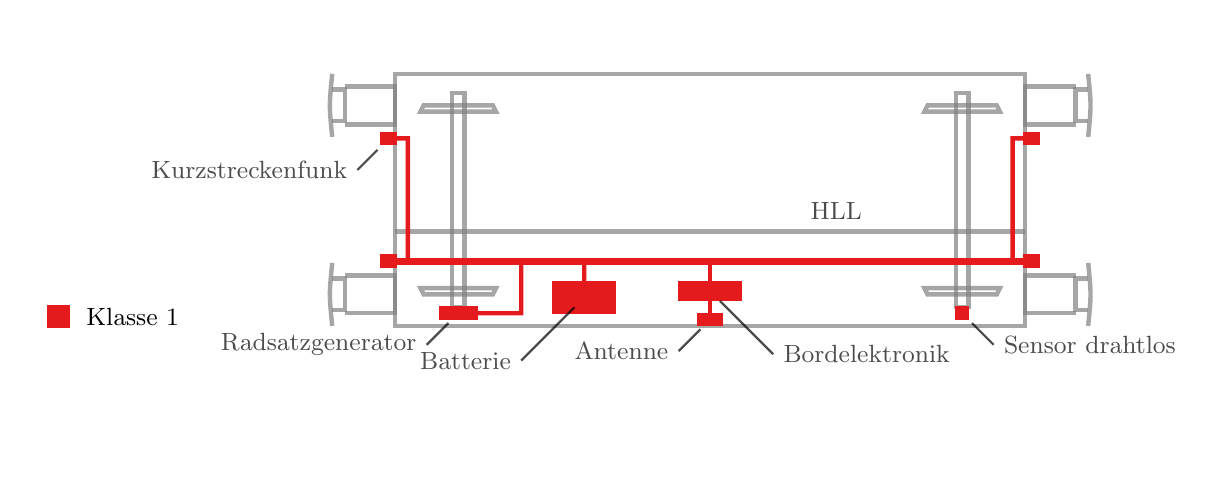
\begin{tikzpicture}[font = \sffamily, scale = 0.8]
\tikzstyle{every node}=[font=\small]
\path[class5, fill = none, draw = none] (-3.3, 1.3) rectangle +(.5,.3) node[pos = 0.5] (dri) {};
\path[annotation, draw = none, opacity = 0] (dri) -- +(1,1) node[right] {Antrieb};
    {%wagon as basis
    \path[wagon] (-5,-2) -- (-5,2) -- (5,2) -- (5,-2) -- cycle;
    % HL
    \path[wagon] (-5,-.5) -- (5,-.5) node[pos = 0.7, above] {HLL};
    % Buffer
    \begin{scope}[shift = {(-5,1.5)}]
    	\path[wagon] (-.8,.3) -- (0,.3) -- (0,-.3) -- (-.8,-.3);
    	\path[wagon] (-1,.25) -- (-.8,.25) -- (-.8,-.25) -- (-1,-.25);
    	\path[wagon] (-1,-.5) .. controls (-1.05,0) and (-1.05,0) .. (-1,.5);
    \end{scope}
    \begin{scope}[shift = {(-5,-1.5)}]
    	\path[wagon] (-.8,.3) -- (0,.3) -- (0,-.3) -- (-.8,-.3);
    	\path[wagon] (-1,.25) -- (-.8,.25) -- (-.8,-.25) -- (-1,-.25);
    	\path[wagon] (-1,-.5) .. controls (-1.05,0) and (-1.05,0) .. (-1,.5);
    \end{scope}
    \begin{scope}[shift = {(5,-1.5)}, rotate = 180]
    	\path[wagon] (-.8,.3) -- (0,.3) -- (0,-.3) -- (-.8,-.3);
    	\path[wagon] (-1,.25) -- (-.8,.25) -- (-.8,-.25) -- (-1,-.25);
    	\path[wagon] (-1,-.5) .. controls (-1.05,0) and (-1.05,0) .. (-1,.5);
    \end{scope}
    \begin{scope}[shift = {(5,1.5)}, rotate = 180]
    	\path[wagon] (-.8,.3) -- (0,.3) -- (0,-.3) -- (-.8,-.3);
    	\path[wagon] (-1,.25) -- (-.8,.25) -- (-.8,-.25) -- (-1,-.25);
    	\path[wagon] (-1,-.5) .. controls (-1.05,0) and (-1.05,0) .. (-1,.5);
    \end{scope}
    %Wheelset
    \begin{scope}[shift = {(-4,0)}]
    	\path[wagon] (-.1,1.7) -- (.1,1.7) -- (.1,-1.7) -- (-.1, -1.7) -- cycle; 
    	\path[wagon] (-.6,1.4) -- (.6,1.4) -- (.55,1.5) -- (-.55, 1.5) -- cycle; 
    	\path[wagon] (-.6,-1.4) -- (.6,-1.4) -- (.55,-1.5) -- (-.55, -1.5) -- cycle; 
    \end{scope}
    \begin{scope}[shift = {(4,0)}]
    	\path[wagon] (-.1,1.7) -- (.1,1.7) -- (.1,-1.7) -- (-.1, -1.7) -- cycle; 
    	\path[wagon] (-.6,1.4) -- (.6,1.4) -- (.55,1.5) -- (-.55, 1.5) -- cycle; 
    	\path[wagon] (-.6,-1.4) -- (.6,-1.4) -- (.55,-1.5) -- (-.55, -1.5) -- cycle; 
    \end{scope}}
    
    % Class 5

    % Class 4

    % Class 3

    %Class 2
    
    {%class 1
    %Tube
    \path[class1] (-5,-1) -- (5,-1);
    \path[class1] (-5,-.95) -- (5,-.95);
    %Short range communication
    \path[class1, fill = class1] (-5.2, -.9) rectangle (-5,-1.05)node[pos = 0.5] (sra) {};
    \path[class1, fill = class1] (5.2, -.9) rectangle (5,-1.05)node[pos = 0.5] (srb) {};
    \path[class1, fill = class1] (5.2, .9) rectangle (5,1.05)node[pos = 0.5] (src) {};
    \path[class1, fill = class1] (-5.2, .9) rectangle (-5,1.05) node[pos = 0.5] (srd) {};
    \path[class1] (srd) +(-.1,0) -- +(.3,0) -- (-4.8,-1);
    \path[class1] (src) +(.1,0) -- +(-.3,0) -- (4.8,-1);
    \path[annotation] (srd) -- +(-.5,-.5) node[left] {Kurzstreckenfunk};
    %Wheelset generator
    \path[class1, fill = class1, thin] (-4.3, -1.9) rectangle +(.6,.2) node[pos = 0.5] (wsg) {};
    \path[class1] (wsg) +(-.1,0) -- +(1,0) -- (-3,-1);
    \path[annotation] (wsg) -- +(-.5,-.5) node[left] {Radsatzgenerator};
    %Wireless sensor
    \path[class1, fill = class1, thin] (3.9, -1.7) rectangle +(.2,-.2) node[pos = 0.5] (wss) {};
    \path[annotation] (wss) -- +(.5,-.5) node[right] {Sensor drahtlos};
    %BCU
    \path[class1, fill = class1, thin] (-.5, -1.6) rectangle +(1,.3) node[pos = 0.5] (bcu) {};
    \path[class1] (bcu) +(0,0)  -- (0,-1);
    \path[annotation] (bcu) -- +(1,-1) node[right] {Bordelektronik};
    %Antenna
    \path[class1, fill = class1, thin] (-.2, -2) rectangle +(.4,.2) node[pos = 0.5] (ant) {};
    \path[class1] (ant) +(0,-.1) -- (bcu) ;
    \path[annotation] (ant) -- +(-.5,-.5) node[left] {Antenne};
    %Battery
    \path[class1, fill = class1, thin] (-2.5, -1.8) rectangle +(1,.5) node[pos = 0.5] (bat) {};
    \path[class1] (bat) +(0,0)  -- (-2,-1);
    \path[annotation] (bat) -- +(-1,-1) node[left] {Batterie};
    }
    
    %Legende
    \begin{scope}[shift = {(1.5,-4)}]
	\path[wagon, opacity = 0] (-12.3, 2.5) rectangle +(2.7,-2.7) node[pos = 0.03, above, anchor = south west] {};
	\path[class1, fill = class1] (-12,2) rectangle +(.3,.3) node[pos = .5, right, label={[shift={(0.8,-.4)}]Klasse 1}] {};
    \end{scope}
    
\end{tikzpicture}
    \caption{Klasse 1 mit Stromversorgung, Telematik und Datenvernetzung - angelehnt an \cite{ETR_3} }
    \label{fig:Klasse1}
\end{figure} 
In der ersten Ausbaustufe, siehe Abbildung \ref{fig:Klasse1}, ist die Anbringung einer Bordelektronik mit  entsprechender Spannungsversorgung geplant. Die Spannungsversorgung kann als Batterie mit Speisung durch einen Achsdeckelgenerator, Solarpanels oder ähnlichem realisiert werden. Auch eine Pufferbatterie mit Speisung durch die Automatische Kupplung ist denkbar. Dazu kommen verschiedene Antennen und Kurzstreckenfunk zur Kommunikation mit anderen Wagen. Auch Sensoren zur Erfassung verschiedener Telematikfunktionen sind geplant.\par
In diesem Stadium ist der Wagen noch nicht 'aktiver' als ein nicht ausgerüsteter Wagen, aber er kann sich mitteilen. Mitteilungen können sein: 
\begin{itemize}
    \item Standort / GPS
    \item (Be-)Ladung
    \item Laufleistung
    \item (ungewöhnliche) Vibrationen (beispielsweise durch Flachstellen)
    \item Heißläuferdedektion
    \item letzte Wartungs- und Instandhaltungsintervalle
    \item Zustand der Bremse
    \item ...
\end{itemize}
Diese Stufe soll im Demonstrator realisiert werden.

\subsubsection{Ausbaustufe 2: Ausbaustufe 1 + Automatisierung der Bremsbedienung}
\begin{figure}[htbp] 
    \input{Bilder/Ausbaustufe_2.tex}
    \caption{Klasse 2 bestehend aus Klasse 1 und der Automatisierung der Bremsbedienung - angelehnt an \cite{ETR_3}}
    \label{fig:Klasse2}
\end{figure} 
In der zweiten Ausbaustufe, siehe Abbildung \ref{fig:Klasse2}, ist eine Aktorik für Endabsperrhähne, Handbremse und Bremsart geplant. Dadurch kann ein Teil der Bremsbedienung so weit automatisiert werden, dass ein Einstellen der Bremsart anhand von anderen Wagen im \gls{Wagenzug}, Gewicht und Bremsfähigkeit möglich ist. Außerdem ist die automatische Parkbremse realisiert.\par
Nach einer vollständigen Zugzusammenstellung kann das System vollständig abgeschaltet und durch einen Wagenmeister abgenommen werden. Sicherheitsfunktionen des Wagens und der Bremse bleiben für Zugfahrten unangetastet. Wichtig dafür ist eine Nutzung von bistabilen Ventilen im System. Diese sorgen für einen sicheren Zustand auch bei abgeschaltetem System und es ist nur ein Nachweis über die Bistabilität dieser zu führen.\par
Ein Ausbau dieser Stufe im Demonstrator ist geplant.

\subsubsection{Ausbaustufe 3: Ausbaustufe 2 + ep-''light''-Bremsen}
\begin{figure}[htbp] 
    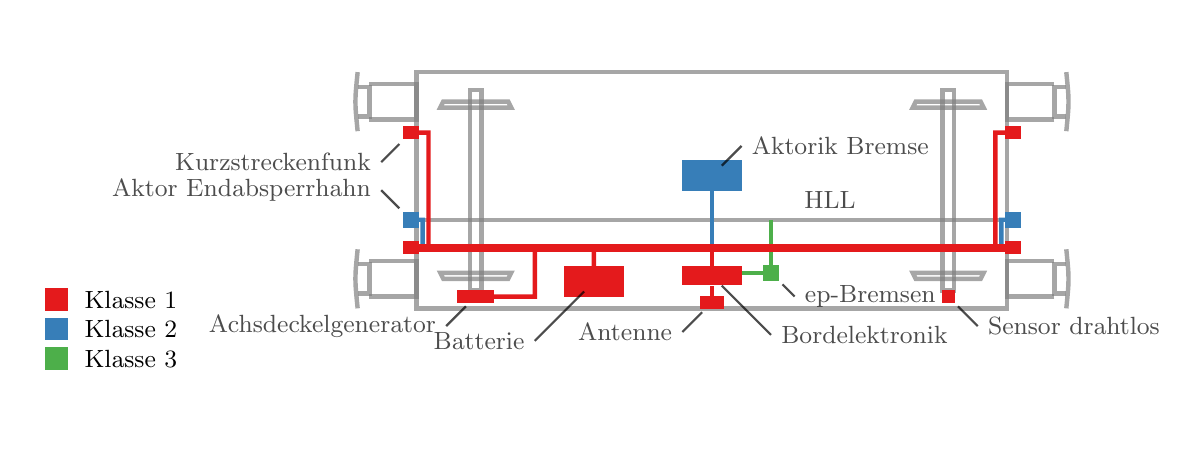
\begin{tikzpicture}[font = \sffamily, scale = 0.75]
\tikzstyle{every node}=[font=\small]
\path[class5, fill = none, draw = none] (-3.3, 1.3) rectangle +(.5,.3) node[pos = 0.5] (dri) {};
\path[annotation, draw = none, opacity = 0] (dri) -- +(1,1) node[right] {Antrieb};
    {%wagon as basis
    \path[wagon] (-5,-2) -- (-5,2) -- (5,2) -- (5,-2) -- cycle;
    % HL
    \path[wagon] (-5,-.5) -- (5,-.5) node[pos = 0.7, above] {HLL};
    % Buffer
    \begin{scope}[shift = {(-5,1.5)}]
    	\path[wagon] (-.8,.3) -- (0,.3) -- (0,-.3) -- (-.8,-.3);
    	\path[wagon] (-1,.25) -- (-.8,.25) -- (-.8,-.25) -- (-1,-.25);
    	\path[wagon] (-1,-.5) .. controls (-1.05,0) and (-1.05,0) .. (-1,.5);
    \end{scope}
    \begin{scope}[shift = {(-5,-1.5)}]
    	\path[wagon] (-.8,.3) -- (0,.3) -- (0,-.3) -- (-.8,-.3);
    	\path[wagon] (-1,.25) -- (-.8,.25) -- (-.8,-.25) -- (-1,-.25);
    	\path[wagon] (-1,-.5) .. controls (-1.05,0) and (-1.05,0) .. (-1,.5);
    \end{scope}
    \begin{scope}[shift = {(5,-1.5)}, rotate = 180]
    	\path[wagon] (-.8,.3) -- (0,.3) -- (0,-.3) -- (-.8,-.3);
    	\path[wagon] (-1,.25) -- (-.8,.25) -- (-.8,-.25) -- (-1,-.25);
    	\path[wagon] (-1,-.5) .. controls (-1.05,0) and (-1.05,0) .. (-1,.5);
    \end{scope}
    \begin{scope}[shift = {(5,1.5)}, rotate = 180]
    	\path[wagon] (-.8,.3) -- (0,.3) -- (0,-.3) -- (-.8,-.3);
    	\path[wagon] (-1,.25) -- (-.8,.25) -- (-.8,-.25) -- (-1,-.25);
    	\path[wagon] (-1,-.5) .. controls (-1.05,0) and (-1.05,0) .. (-1,.5);
    \end{scope}
    %Wheelset
    \begin{scope}[shift = {(-4,0)}]
    	\path[wagon] (-.1,1.7) -- (.1,1.7) -- (.1,-1.7) -- (-.1, -1.7) -- cycle; 
    	\path[wagon] (-.6,1.4) -- (.6,1.4) -- (.55,1.5) -- (-.55, 1.5) -- cycle; 
    	\path[wagon] (-.6,-1.4) -- (.6,-1.4) -- (.55,-1.5) -- (-.55, -1.5) -- cycle; 
    \end{scope}
    \begin{scope}[shift = {(4,0)}]
    	\path[wagon] (-.1,1.7) -- (.1,1.7) -- (.1,-1.7) -- (-.1, -1.7) -- cycle; 
    	\path[wagon] (-.6,1.4) -- (.6,1.4) -- (.55,1.5) -- (-.55, 1.5) -- cycle; 
    	\path[wagon] (-.6,-1.4) -- (.6,-1.4) -- (.55,-1.5) -- (-.55, -1.5) -- cycle; 
    \end{scope}}
    
    % Class 5

    % Class 4

    % Class 3
    {
    \path[class3] (1,-.5) -- (1,-1.3);
    \path[class3, fill = class3] (.9,-1.3) rectangle (1.1,-1.5) node[pos = 0.5] (epb) {};
    \path[class3] (epb) +(.1,0) -- +(-.5,0);
    \path[annotation] (epb) -- +(.4,-.4) node[right] {ep-Bremsen};
    }
    %Class 2
    {%End cocks
    \path[class2, fill = class2] (-5.2, -.4) rectangle (-5,-.6) node[pos = 0.5] (eca) {};
    \path[class2, fill = class2] (5.2, -.4) rectangle (5,-.6) node[pos = 0.5] (ecb) {};
    \path[class2] (eca) +(-.1,0) -- +(.2,0) -- (-4.9,-1);
    \path[class2] (ecb) +(.1,0) -- +(-.2,0) -- (4.9,-1);
    \path[annotation] (eca) -- +(-.5,.5) node[left] {Aktor Endabsperrhahn};
    %Battery
    \path[class2, fill = class2, thin] (-.5, 0) rectangle +(1,.5) node[pos = 0.5] (bcu) {};
    \path[class2] (bcu) +(0,0)  -- (0,-1);
    \path[annotation] (bcu) -- +(.5,.5) node[right] {Aktorik Bremse};
    }
    
    {%class 1
    %Tube
    \path[class1] (-5,-1) -- (5,-1);
    \path[class1] (-5,-.95) -- (5,-.95);
    %Short range communication
    \path[class1, fill = class1] (-5.2, -.9) rectangle (-5,-1.05)node[pos = 0.5] (sra) {};
    \path[class1, fill = class1] (5.2, -.9) rectangle (5,-1.05)node[pos = 0.5] (srb) {};
    \path[class1, fill = class1] (5.2, .9) rectangle (5,1.05)node[pos = 0.5] (src) {};
    \path[class1, fill = class1] (-5.2, .9) rectangle (-5,1.05) node[pos = 0.5] (srd) {};
    \path[class1] (srd) +(-.1,0) -- +(.3,0) -- (-4.8,-1);
    \path[class1] (src) +(.1,0) -- +(-.3,0) -- (4.8,-1);
    \path[annotation] (srd) -- +(-.5,-.5) node[left] {Kurzstreckenfunk};
    %Wheelset generator
    \path[class1, fill = class1, thin] (-4.3, -1.9) rectangle +(.6,.2) node[pos = 0.5] (wsg) {};
    \path[class1] (wsg) +(-.1,0) -- +(1,0) -- (-3,-1);
    \path[annotation] (wsg) -- +(-.5,-.5) node[left] {Achsdeckelgenerator};
    %Wireless sensor
    \path[class1, fill = class1, thin] (3.9, -1.7) rectangle +(.2,-.2) node[pos = 0.5] (wss) {};
    \path[annotation] (wss) -- +(.5,-.5) node[right] {Sensor drahtlos};
    %BCU
    \path[class1, fill = class1, thin] (-.5, -1.6) rectangle +(1,.3) node[pos = 0.5] (bcu) {};
    \path[class1] (bcu) +(0,0)  -- (0,-1);
    \path[annotation] (bcu) -- +(1,-1) node[right] {Bordelektronik};
    %Antenna
    \path[class1, fill = class1, thin] (-.2, -2) rectangle +(.4,.2) node[pos = 0.5] (ant) {};
    \path[class1] (ant) +(0,-.1) -- (bcu) ;
    \path[annotation] (ant) -- +(-.5,-.5) node[left] {Antenne};
    %Battery
    \path[class1, fill = class1, thin] (-2.5, -1.8) rectangle +(1,.5) node[pos = 0.5] (bat) {};
    \path[class1] (bat) +(0,0)  -- (-2,-1);
    \path[annotation] (bat) -- +(-1,-1) node[left] {Batterie};
    }
    
    %Legende
    \begin{scope}[shift = {(0.75,-4)}]
	\path[wagon, opacity = 0] (-12.3, 2.5) rectangle +(2.7,-2.7) node[pos = 0.03, above, anchor = south west] {};
	\path[class1, fill = class1] (-12,2) rectangle +(.3,.3) node[pos = .5, right, label={[shift={(0.8,-.4)}]Klasse 1}] {};
	\path[class2, fill = class2] (-12,1.5) rectangle +(.3,.3) node[pos = .5, right, label={[shift={(0.8,-.4)}]Klasse 2}] {};
	\path[class3, fill = class3] (-12,1) rectangle +(.3,.3) node[pos = .5, right, label={[shift={(0.8,-.4)}]Klasse 3}] {};
    \end{scope}
    
\end{tikzpicture}
    \caption{Klasse 3 bestehend aus Klasse 2 und der eingeführten ep-''light''-Bremse - angelehnt an \cite{ETR_3}}
    \label{fig:Klasse3}
\end{figure} 
In der dritten Ausbaustufe, siehe Abbildung \ref{fig:Klasse3}, kommt zusätzlich zur Bremsbedienung auch eine Vorform der \gls{ep-Bremse} hinzu: die ep-''light''-Bremse. Diese sorgt für kürzere Bremswege und weniger Verschleiß, weil der Bremseinsatz über die gesamte Zuglänge synchron erfolgt. Weil sie aber nicht auf die Bremshunderstel angerechnet wird, sind die sicherheitstechnsichen Anforderungen noch überschaubar. Im Gegensatz zur "`vollwertigen"' aus dem Personenverkehr bekannten ep-Bremse muss auf die Hauptbehälterleitung HBL verzichtet werden. Daher hat ep-light auf das Lösen der Bremse keinen Einfluss.\par
%Dafür muss dieses System richtig eingestellt werden. 
Die ep-Bremse ist die erste Güterwagen 4.0-Komponente, die auch bei Zugfahrten eingeschaltet bleibt. Diese Stufe wird im Demonstrator realisiert.

\subsubsection{Ausbaustufe 4: Ausbaustufe 3 + automatisierter Zugschluss}
\begin{figure}[htbp] 
    \input{Bilder/Ausbaustufe_4.tex}
    \caption{Klasse 4 bestehend aus Klasse 3 und der Automatisierung des Zugschlusses - angelehnt an \cite{ETR_3}}
    \label{fig:Klasse4}
\end{figure} 
In der vierten Ausbaustufe, siehe Abbildung \ref{fig:Klasse4}, ist unter anderem ein technisch gesicherter Zugschluss geplant. Damit können auch für Güterzüge Zugsicherungsverfahren, die eine technische Überwachung der Zugintegrität voraussetzen (ETCS Level 3, PTC), realisiert werden. Gleichzeitig wird das für die Rückfallebene notwendige Zugschlusssignals am letzten Wagen durch eine elektrische Leuchte ersetzt.\par
%Heute muss die Zugschlusstafel noch manuell gesteckt werden. Dazu muss eine Person den gesamten Zug von bis zu 700 m ablaufen um die die entsprechenden Signale am letzten Wagen anzubringen.\par
%Vor allem aber soll diese Funktion aber den Mehrwert der technischen Sicherheit bei der Zugintigrität bieten. Durch eine Integration eines echtzeitfähigem Zugschlusses bietet diese Funktion eine durchgängige Möglichkeit der Zugintigrität.\par
%Damit ist in Zukunft auch eine Fahrt von Güterzügen in ETCS Level 3 möglich.\par
Diese Stufe soll nicht im Projekt angegangen werden.

\subsubsection{Ausbaustufe 5: Ausbaustufe 4 + Rangierantrieb} \label{sec:A5}
\begin{figure}[htbp] 
    \input{Bilder/Ausbaustufe_5.tex}
    \caption{Klasse 5 bestehend aus Klasse 4 und einem Rangierantrieb - angelehnt an \cite{ETR_3}}
    \label{fig:Klasse5}
\end{figure}
In der fünften Ausbaustufe, siehe Abbildung \ref{fig:Klasse5}, kommt der Rangierantrieb mit einer Vielzahl weiterer technischer Komponenten und einer zusätzlichen Stromversorgung hinzu. %dieser kann allerdings auch bereits auf einen Wagen der nur mit Stufe 1 und 2 ausgestattet ist aufgesetzt werden. Damit dieser ohne Probleme funktioniert braucht er neben einem Antrieb zusätzlich eine weitere Batterie und Umrichter. Zur Speisung der zweiten Batterie wird auch ein zweiter Radsatzgenerator benötigt.\par
%In diesem Stadium kann von einem automatisierten Güterwagen gesprochen werden. 
Ein so ausgestatteter Wagen kann selbstständig bei der ''Briefkastenbedienung'' (siehe \cite{GAK}) assistieren und auf dem Werksgelände ohne Rangierlok oder andere Verschiebeeinheiten verfahren.\par
Die Umsetzung dieser Stufe ist nicht im Projekt geplant.

\subsection{Abgrenzung des Güterwagen 4.0 vom konventionellen Güterwagen}
\subsubsection{Leistungsniveau und Energieversorgung}
Die Stromversorgung soll in diesem Projekt nur für ein geringes Leistungsniveau bereitstehen. Es ist keine Anwendung mit größerer Stromzufuhr geplant. Ein später folgender \gls{Gueterwagen 40}  kann dies aber eventuell fordern.\par
In diesem Projekt wird weder die Energieversorgung des späteren 'vollständig' ausgebauten \gls{Gueterwagen 40} noch die Energieversorgung nach der VDI-Richtlinie 5905 entwickelt. Dabei wird es wahrscheinlich Überschneidungen geben, auch werden Erfahrungen aus den Arbeitsrunden mitgenommen und einfließen, aber es wird keine exemplarische Realisierung dessen.\par
Eine vollständige Stromversorgung nach der VDI-Richtlinie 5905 oder ein Prototyp der diese Richtlinie prägt, soll nicht entstehen. 

\subsubsection{Bremse}
Die Bremse stellt, neben dem Bordrechner, ein Herzstück des \gls{Gueterwagen 40}  dar.
Hier ist eine Teilautomatisierung der Bremse im Bereich der Hauptluftleitung, Bremsumsteller, \gls{Lastwechsel} und Feststellbremse geplant. Diese soll mit Aktoren automatisch oder auf Befehl umgestellt werden. Dadurch soll auch eine automatische Bremsprobe und eine automatische Bremsberechnung möglich sein. Ebenso eine Stillstandsüberwachung.\par
Nicht geplant ist dagegen eine automatische Notbremsfunktion, die beispielsweise die Handbremse anlegt, wenn ein Hindernis auftaucht. Dies ist als Aufbau möglich, soll aber nicht zur Standardausrüstung gehören. Auch eine entsprechende wirtschaftliche Betrachtung findet nicht statt.\par
%Während dieses Projektes ist eine Ausstattung der Wagen mit einer ep-''light''-Bremse als Versuch geplant. Diese wird allerdings ohne Anrechnung auf die Bremsleistung im Testbetrieb stattfinden, sodass eine erste Einführung probehalber unkritisch ist. Eine angerechnete ep-Bremse im Güterverkehr wäre aus vielen Gründen sehr interessant, muss allerdings aus Sicherheitsgründen weitreichender geplant sein.\par

\subsubsection{Intelligente Vernetzung}
Der \gls{Gueterwagen 40} ist als 'intelligenter' Wagen im Sinne der Industrie 4.0 im Schienenverkehr geplant. Dafür benötigt er, neben der Energieversorgung und der teilautomatisierten Bremse, auch einen Bordrechner, der diese 'Intelligenz' liefert.\par
Auf diesem Rechner soll als Betriebssystem das sogenannte 'WagonOS' installiert sein. Dieses bietet als Open Source-System ein offenes Betriebssystem mit vielen Ausbaumöglichkei- ten. Das WagonOS bietet den Nutzern des \gls{Gueterwagen 40}  diesen auf genau die benötigten Anwendungsfälle zu Optimieren und sogar die Möglichkeit eigene Applikationen zu erstellen.\par
Des Weiteren liegen auf dieser Speichereinheit dezentral alle für die Zugbildung und Instandhaltung wichtigen Informationen über den Wagen. Dazu gehören bauartspezifische Parameter wie Gewicht, Länge, Achszahl, maximal Zuladung und Höchstgeschwindigkeit genauso wie wagenspezifische Informationen wie Besitzer, Laufleistung, Informationen aus den Sensoren, letzte Wartungen und nächste Instandhaltungszyklen.\par
Diese Informationen liegen ebenso als 'Digitaler Zwilling' in einer Cloud. Bei Verbindung des Wagens zum Internet und Änderung der Informationen auf dem Wagen wird dieser Zwilling regelmäßig aktualisiert.\par
Im Verband mit anderen Wagen verhält sich der \gls{Gueterwagen 40} 'sozial' und teilt alle notwendigen Informationen über sich mit den anderen Wagen und der Lok als gleichberechtigte Partner. Durch die Verbindung von Wagen zu Wagen ist keine durchgehende Internetverbindung notwendig. Die Informationen können lokal ausgetauscht und später synchronisiert werden.\par
Im Projekt umgesetzt werden soll davon eine reduzierte Form des WagonOS. Eine Entwicklung des vollständigen Betriebssystems findet nicht im Rahmen dieses Projektes statt.\par
Diese reduzierte Form des Betriebssystems soll eine Speicherung und Auswertung aller relevanter Daten auf dem Bordrechner ermöglichen. Eine weitere Datenspeicherung als 'Digitaler Zwilling' findet in der Cloud statt.

\subsubsection{Beladung und Ladungssicherung}
Bei der Beladung und Ladungssicherung ist es möglich diverse Sensoren, auch unabhängig von der Beladung mit palettiertem Gut, zum Beispiel für Hafenverkehr einzubauen und zu überwachen. Beispiele dafür sind:
\begin{itemize}
    \item Königszapfen bei Taschenwagen
    \item Ladeebenenverstellung bei der Automobilverladung
    \item Tragzapfenverstellung bei Containertragwagen
    \item Ladungssicherung von Coiltransportern
    \item Verstellbare und verschließbare Trennwände bei Schiebewandwagen
    \item Technische Überwachung von diversen Hebeln und Schaltern
    \item Temperatursensoren an temperaturempfindlichem Gut
    \item ...
\end{itemize}
Auch möglich ist es Spanngurte mit Sensoren in den Textilien zu entwickeln, die über Funkverbindung mit dem Wagen kommunizieren können.\par
Diese Sensoren können mittels Funkkommunikation oder mittels Datenleitung ausgelesen werden. Hier ist auf eine sichere Übertragung zu achten (vgl. dazu auch ITSS\footnote{Industrieplattform Telematik und Sensorik im Schienengüterverkehr} Schnittstelle 2\footnote{Datenaustausch zwischen Telematikgeräten und Sensoren}).\par
Im Rahmen des Projektes sollen diese Punkte nicht umgesetzt werden.

\subsection{Weitere Möglichkeiten}
Die durch die Stromversorgung und das offene Betriebssystem ermöglichten Aussichten sind quasi grenzenlos.\par
Es sind beispielsweise Warnlichter oder Rundumlichter bei der Bewegung des Güterwagens möglich, der Einbau einer Alarmanlage oder auch 'nur' Akustikfunktionen bei Bewegung.\par
Ebenfalls möglich ist eine ansetzbare Front- oder Rückfahrkamera für Fahrer eines Zweiwegefahrzeuges auf LKW-Basis oder das bereits vorgestellte Prinzip der technisch über- wachten Spitze von Rangierabteilungen\cite{RTUS} ist möglich.\par
Ebenso möglich sind auch für Unternehmen angepasste Applikationen für Kommunikation mit einzelnen Toren, Kränen oder Beladungsstationen.\par
Diese Punkte werden im Rahmen des Projektes jedoch nicht umgesetzt.
